
\ifspanish

\else

A game has three players, named $G_0$, $G_1$ and $G_2$ and consists of a sequence of rounds. At each round, only one of the players enters the game. 

The result of each round can be win or lose. If the active player wins a round, she can play the next one. If she loses, she must pass the turn to one of the other players, which is chosen at random with equal probabilities.

Based on the game skills of the players, it is known that the winning probabilities are 0.4 (for $G_0$), 0.6 ($G_1$) and 0.8 ($G_2$).

Let $X_k$ be the one-sided stochastic process that represents the sequence of active players during a game, such that $X_k=i$ means that the active player at time $k$ is $G_i$.

The game always starts with player 0, that is, $X_0=0$.
\begin{parts}
\part [4] Formulate the problem as a stationary Markov chain: compute the transition matrix and draw the transition graph.
\part[4] Compute the probability that the first players in the sequence are $0, 1, 2, 1$ (i.e., $P\{X_0=0, X_1=1, X_2=2, X_3=1)$).
\part[5] Compute $P\{X_2=1\}$.
\part[5] Compute the stationary distribution
\part[5] Players $G_0$ and $G_1$ are unsatisfied because $G_2$, with better skills, plays most rounds. They decide to make the game fairer, in the sense that, in the long term, everyone plays with the same frequency. To do so, they proceed as follows: 
\begin{enumerate}
\item If $G_0$ is the active player and loses, she passes the turn to player $G_1$ with probability $q$ and to $G_2$ with probability $1-q$.
\item If $G_1$ is the active player and loses, she passes the turn to player $G_0$ with probability $r$ and to $G_2$ with probability $1-r$.
\end{enumerate}
Determine if $G_0$ and $G_1$ will succed in making a fair game, that is, if there exist values $q$ and $r$ so that the stationary distribution is uniform, i.e., $\boldsymbol{\pi}= (\frac13, \frac13, \frac13)$ If so, compute them.
\end{parts}

\begin{solution}
\begin{parts}
\part The transition matrix is
\begin{align*}
{\bf P} = \begin{pmatrix}
   0.4  & 0.3 & 0.3  \\
   0.2  & 0.6 & 0.2  \\
   0.1  & 0.1 & 0.8
\end{pmatrix}
\end{align*}
The transition graph is shown in the figure.

{\centering 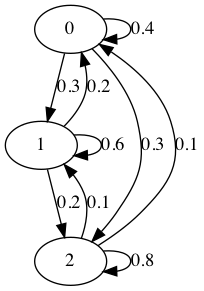
\includegraphics[scale=0.3]{db/figs/SP_202205_markov_chain.png}}

\part Since $X_k$ is a Markov chain
\begin{align*}
P\{X_0 &=0, X_1 =1, X_2=2, X_3=1\}   \\
	&= P\{X_0=0\} P\{X_1=1|X_0=0\} P\{X_2=2| X_1=1\} P\{X_3=1|X_2=2\}    \\
	&= 1 \cdot 0.3 \cdot 0.2 \cdot 0.1 = 0.006
\end{align*}

\part At time $k=2$, we have 
\begin{align*}
P\{X_2=1\} 
   &= \begin{pmatrix} 0 & 1 & 0 \end{pmatrix} 
      {\bf P}^\intercal {\bf P}^\intercal 
      \begin{pmatrix} 1 \\ 0 \\ 0 \end{pmatrix} 
    = \begin{pmatrix} 0.3 & 0.6 & 0.1 \end{pmatrix} 
      \begin{pmatrix} 0.4 \\ 0.3 \\ 0.3 \end{pmatrix} 
%    = 0.12 + 0.18 + 0.03 
    = 0.33
\end{align*}

\part The stationary distribution is the solution of
\begin{align*}
\begin{pmatrix}
   0.4 & 0.2 & 0.1 \\
   0.3 & 0.6 & 0.1 \\
   0.3 & 0.2 & 0.8 \\
   1   & 1   & 1 
\end{pmatrix}
\begin{pmatrix} \pi_0 \\ \pi_1 \\ \pi_2 \end{pmatrix} = 
\begin{pmatrix} \pi_0 \\ \pi_1 \\ \pi_2  \\ 1 \end{pmatrix}
\end{align*}
Since the first 3 equations are linearly dependent, we can remove the first one, 
\begin{align*}
\begin{pmatrix}
   1   &  1   & 1  \\
   0.3 & -0.4 & 0.1  \\
   0.3 &  0.2 & -0.2
\end{pmatrix}
\begin{pmatrix} \pi_0 \\ \pi_1 \\ \pi_2 \end{pmatrix} = 
\begin{pmatrix} 1     \\ 0     \\ 0     \end{pmatrix}
\end{align*}
%which is equivalent to
%\begin{align*}
%\begin{pmatrix}
%   1 &  1   &  1   \\
%   0 & -0.7 & -0.2 \\
%   0 & -0.1 & -0.5 
%\end{pmatrix}
%\begin{pmatrix} \pi_0 \\ \pi_1 \\ \pi_2 \end{pmatrix} = 
%\begin{pmatrix} 1     \\ -0.3  \\ -0.3  \end{pmatrix}
%\end{align*}
%which is equivalent to
%\begin{align*}
%\begin{pmatrix}
%   1 & 1   & 1   \\
%   0 & 0.1 & 0.5 \\
%   0 & 0.7 & 0.2
%\end{pmatrix}
%\begin{pmatrix} \pi_0 \\ \pi_1 \\ \pi_2 \end{pmatrix} = 
%\begin{pmatrix} 1     \\ 0.3   \\ 0.3   \end{pmatrix}
%\end{align*}
%which is equivalent to
%\begin{align*}
%\begin{pmatrix}
%   1 &  1   & 1   \\
%   0 &  0.1 & 0.5 \\
%   0 &  0   & -3.3
%\end{pmatrix} 
%\begin{pmatrix} \pi_0 \\ \pi_1 \\ \pi_2 \end{pmatrix} = 
%\begin{pmatrix} 1     \\ 0.3   \\ -1.8  \end{pmatrix}
%\end{align*}
Therefore:
\begin{align*}
\begin{pmatrix} \pi_0 \\ \pi_1 \\ \pi_2 \end{pmatrix} = 
\frac{1}{11}
\begin{pmatrix} 2 \\ 3 \\ 6 \end{pmatrix}
\end{align*}

\part If the stationary distribution is uniform, we have
\begin{align*}
\begin{pmatrix}
   0.4       & 0.4 r    & 0.1 \\
   0.6 q     & 0.6      & 0.1 \\
   0.6 (1-q) & 0.4(1-r) & 0.8
\end{pmatrix}
\begin{pmatrix} \tfrac13 \\ \tfrac13 \\ \tfrac13 \end{pmatrix} = 
\begin{pmatrix} \tfrac13 \\ \tfrac13 \\ \tfrac13 \end{pmatrix}
\end{align*}
Using the first to equations, we have
\begin{align*}
0.4   + 0.4 r + 0.1 = 1  \\
0.6 q + 0.6   + 0.1 = 1
\end{align*}
The unique solution is $q=0.5$, $r=1.25$. Since $r$ is not a probability value, there is no way to make the game fair.

\end{parts}
\end{solution}


\fi